\section{System Design and Algorithms} \label{sec:Algorithms}

\begin{figure}
\centering
    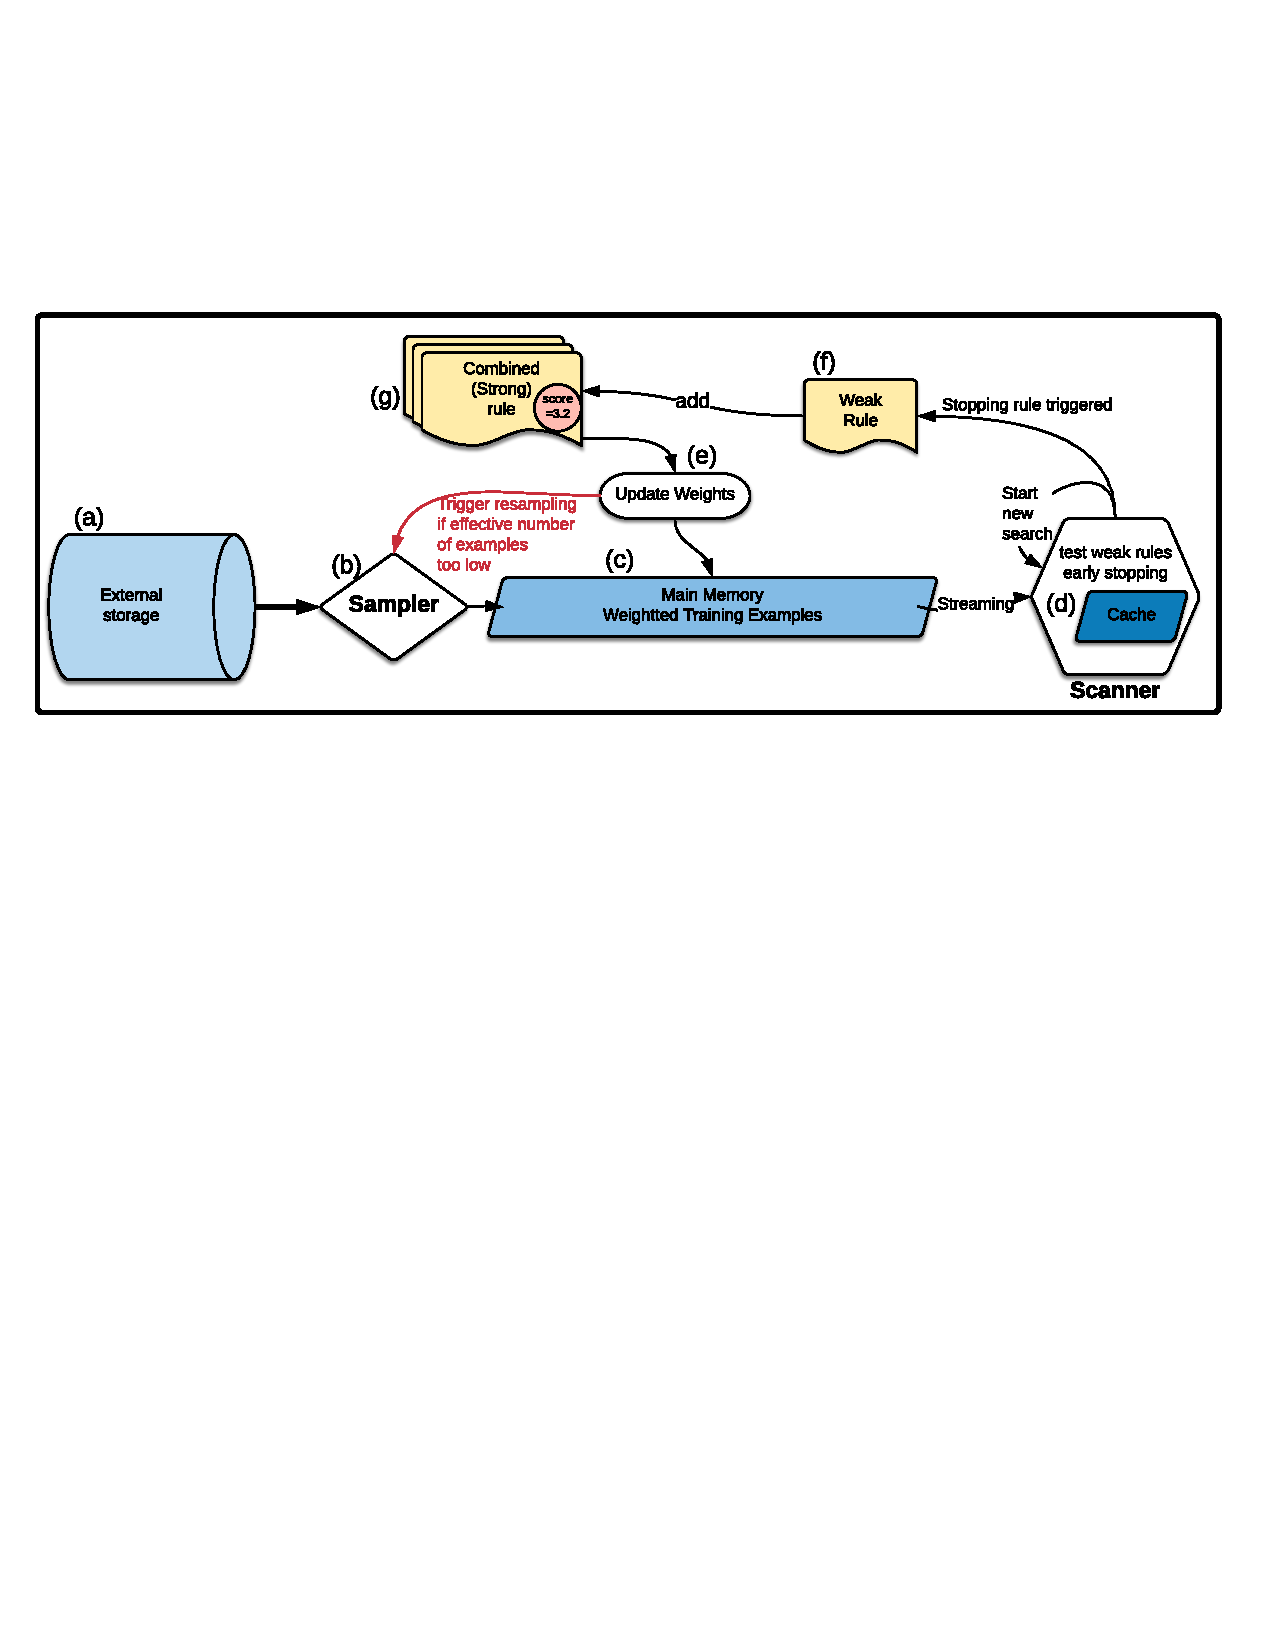
\includegraphics[width=0.5\textwidth]{figs/SingleMachine.pdf}
    \caption{The \Sparrow\ system architecture.}\label{fig:architecture}
    \vspace{0pt}
%\end{minipage}
\end{figure}

The main procedure of \Sparrow\ is for identifying a rule that has a significant
edge (Equation~\ref{eqn:true-edge}). There are two
subroutines that can execute in parallel in the process: a {\bf Scanner (d)} and a
{\bf Sampler (b)}. We describe each subroutine in turn.


\subsection*{Scanner}

The task of a scanner (element {\bf (d)} in Figure~\ref{fig:architecture})
is to read training examples sequentially and stop
when it has identified one of the rules to be a {\em good} rule. More
specifically, at any time point the scanner stores the current strong
rule $H_t$, a set of candidate weak rules $\weakRules$ (which
define the candidate strong rules), and a target
edge $\gamma_t$. The scanner scans the training examples stored in
memory sequentially, one at a time. It computes the weight of the
examples using $H_t$ and then updates a running estimate of the edge
of each weak rule $h \in \weakRules$.

The scan stops when the stopping rule determine that
the true edge of a particular weak rule
$\gamma(h_t)$ is, with high probability,
larger than a threshold $\gamma$. The
worker then adds the identified weak rule $h_t$ {\bf (f)} to the current
strong rule $H_t$ to create a new strong rule $H_{t+1}$ {\bf (g)}.
The weight of the added rule is calculated assuming that its edge is
equal to $\gamma$.

The scanner falls into the \textit{Failed} status if after exhausting
all examples in the current sample set, no weak rule with an advantage
larger than the threshold $\gamma$ is detected.
When it happens, \Sparrow\ shrinks the value of the target advantage
threshold $\gamma$ and restart the scanner.
In practice, \Sparrow\ keeps track of the empirical edges $\edgeEmp{(h)}$
of all weak rules $h$.
When the failure status happens, it reset the threshold $\gamma$
to be just below the value of the current maximum empirical edge of
all weak rules (Figure~\ref{fig:edge}).

\begin{figure}
\centering
    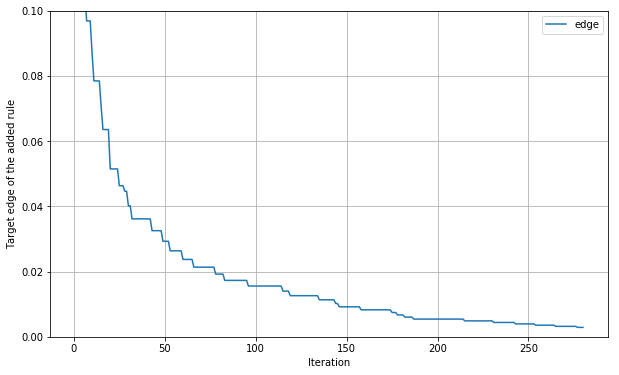
\includegraphics[width=0.5\textwidth]{figs/edge.png}
    \caption{The edge of the rules being added to the strong rule
    (trained on the splice site dataset).
    New rules are being added to the ensemble with a weight calculated
    using the value of the threshold $\gamma$ at the time of their
    detection until no rule with an advantage over $\gamma$ can be detected.
    At that time \Sparrow\ shrinks the value of the target edge $\gamma$,
    and restarts the scanner.\label{fig:edge}}
    \vspace{0pt}
\end{figure}


\subsection*{Sampler}

Our assumption is that the entire training dataset does
not fit into main memory and is therefore stored in external storage
{\bf (a)}. As boosting progresses, the weights of the examples become
increasingly skewed, making the dataset in memory effectively smaller.
To counteract that skew, {\bf Sampler} prepares a {\em new}
training set, in which all of the examples have equal weight, by using
selective sampling. When the effective sample size associated
with the old training set becomes too small, the scanner stops using
the old training set and starts using the new one.\footnote{The
  sampler and scanner can run in parallel on separate cores. However in
  our current implementation the worker alternates between scanning and
  sampling.}

The sampler uses selective sampling by which we mean that the
probability that an example $(x,y)$ is added to the sample is
proportional to $w(x,y)$. Each added example is assigned an initial
{\bf weight} of $1$.
{There are several known algorithms
  for selective sampling. The best known one is rejection sampling
  where a biased coin is flipped for each example. We use a method
  known as \textit{minimal variance sampling}~\cite{kitagawa_monte_1996}
  because it produces less variation in the sampled set.}
  
\paragraph*{Incremental Updates} Our experience shows that the most
time consuming part of our algorithms is the computation of the
predictions of the strong rules $H_t$. A natural way to reduce this
computation is to perform it incrementally. In our case this is
slightly more complex than in XGBoost or LightGBM, because {\bf
  Scanner} scans only a  fraction of the examples at each
iteration. To implement incremental update we store for each example,
whether it is on disk or in memory, the results of the latest
update. Specifically, we store for each training example the tuple
$(x, y, w_s, w_l,H_l)$, Where $x,y$ are the feature vector and the
label, $H_l$ is the strong rule last used to calculate the weight of
the example. $w_l$ is the weight last calculated, and $w_s$ is
example's weight when it was last sampled by the sampler. In this way
{\bf Scanner} and {\bf Sampler} share the burden of computing
the weights, a cost that turns out to be the lion's share of the total
run time for our system.




